\documentclass{standalone}
\usepackage{tikz}
\usetikzlibrary{patterns, positioning}
\usepackage[sfdefault]{ClearSans} %% option 'sfdefault' activates Clear Sans as the default text font
\usepackage[T1]{fontenc}

\begin{document}
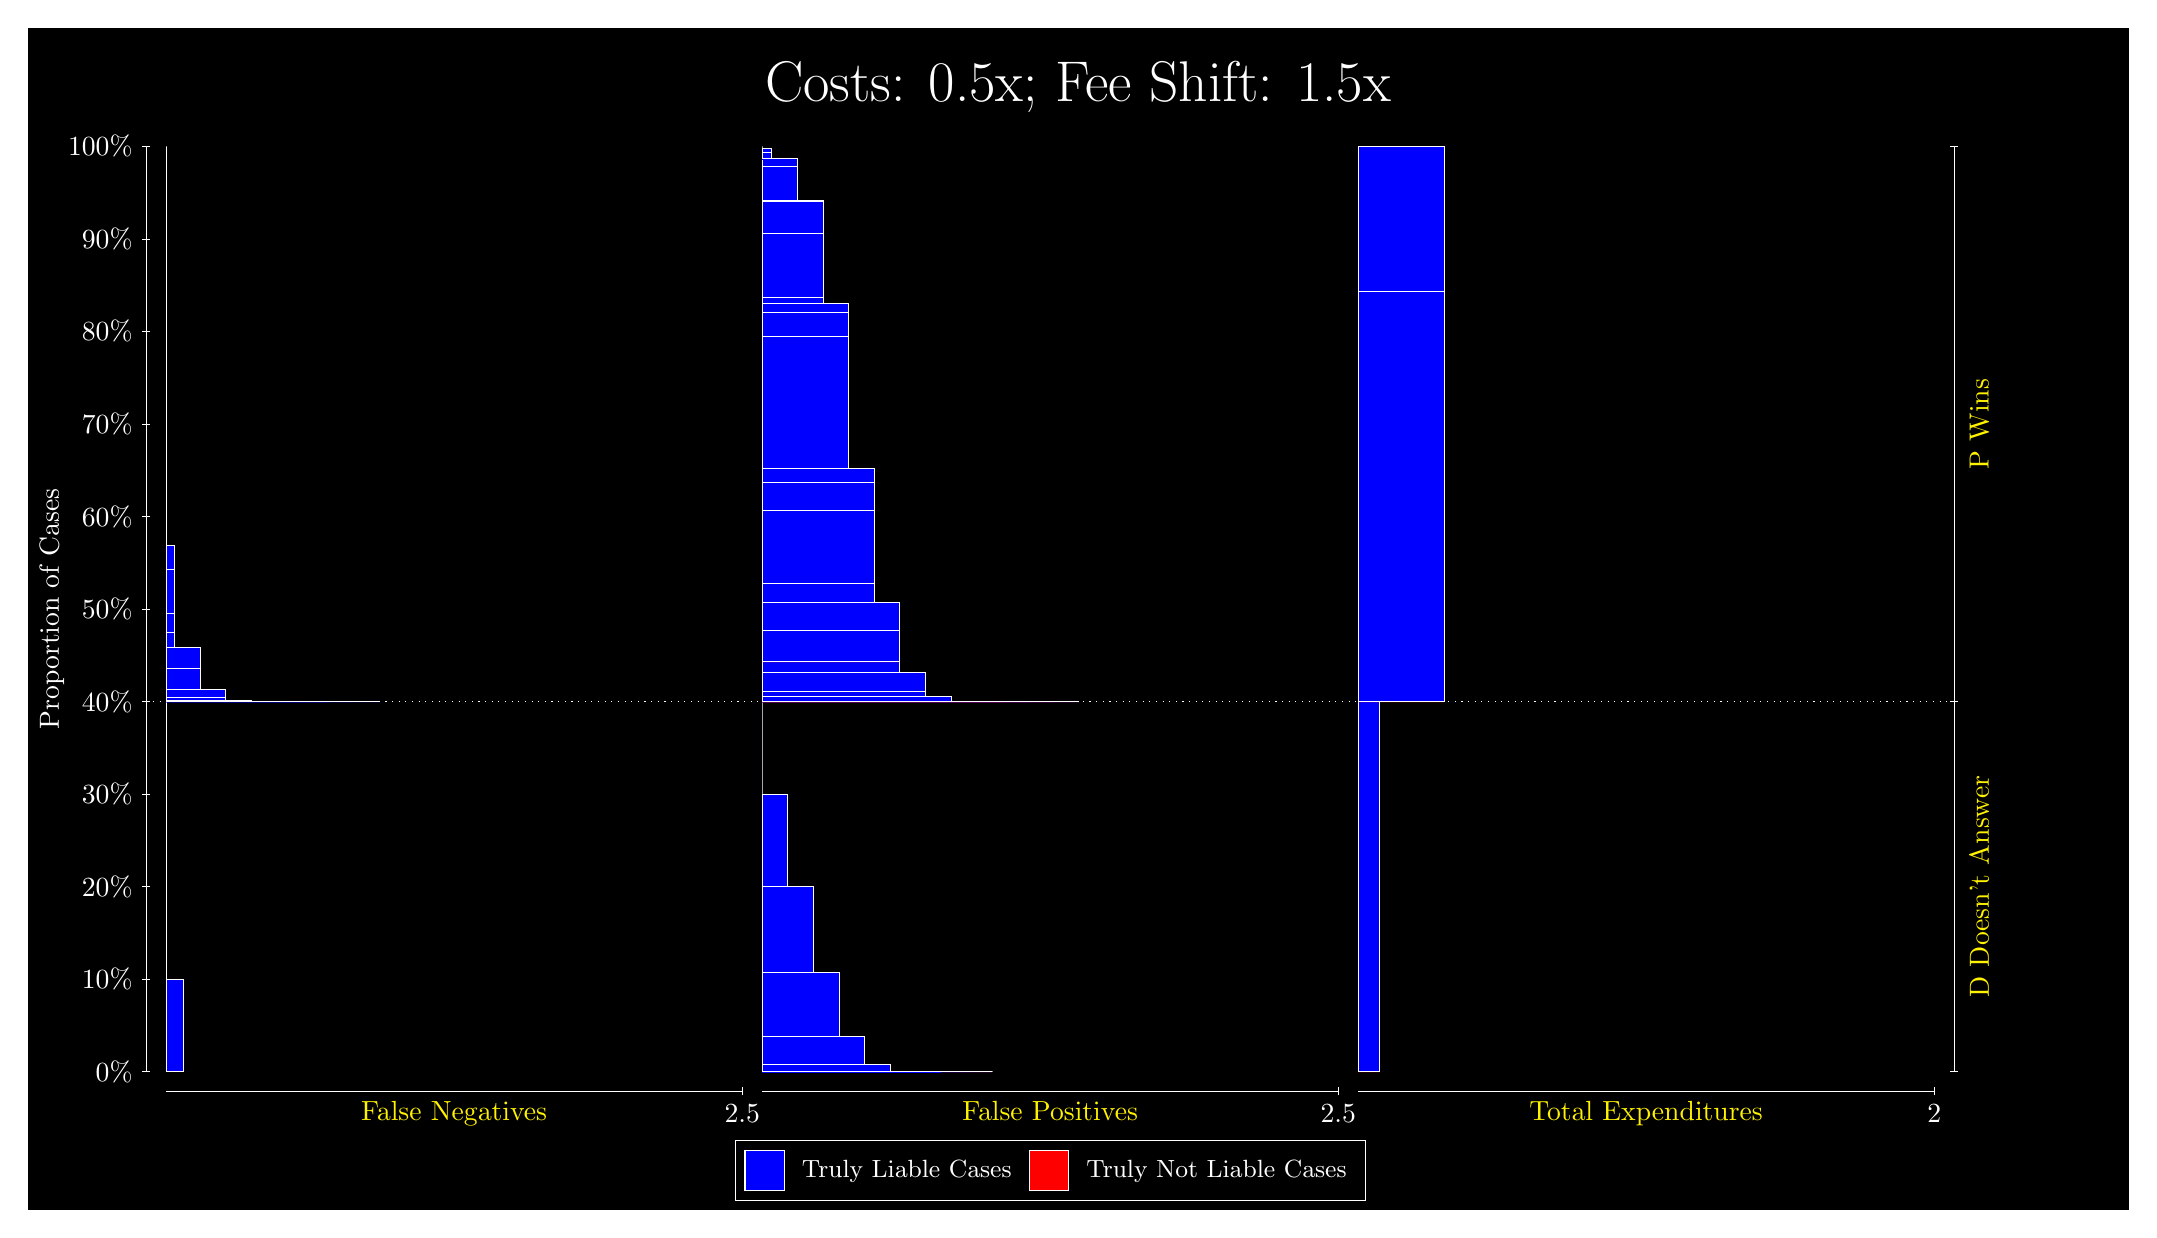
\begin{tikzpicture}
\draw[fill=black] (0,0) rectangle (26.667,15);
\draw[text=white] (0,13.5) rectangle (26.667,15) node[midway] {\huge Costs: 0.5x; Fee Shift: 1.5x};
\draw[white, very thin] (1.5,1.75) -- (1.5,13.5);
\node[rotate=90, text=white, anchor=center] at (0.3, 7.625) {Proportion of Cases};
\draw[white, very thin] (1.45,1.75) -- (1.55,1.75);
\node[text=white, anchor=east] at (1.45, 1.75) {0\%};
\draw[white, very thin] (1.45,2.925) -- (1.55,2.925);
\node[text=white, anchor=east] at (1.45, 2.925) {10\%};
\draw[white, very thin] (1.45,4.1) -- (1.55,4.1);
\node[text=white, anchor=east] at (1.45, 4.1) {20\%};
\draw[white, very thin] (1.45,5.275) -- (1.55,5.275);
\node[text=white, anchor=east] at (1.45, 5.275) {30\%};
\draw[white, very thin] (1.45,6.45) -- (1.55,6.45);
\node[text=white, anchor=east] at (1.45, 6.45) {40\%};
\draw[white, very thin] (1.45,7.625) -- (1.55,7.625);
\node[text=white, anchor=east] at (1.45, 7.625) {50\%};
\draw[white, very thin] (1.45,8.8) -- (1.55,8.8);
\node[text=white, anchor=east] at (1.45, 8.8) {60\%};
\draw[white, very thin] (1.45,9.975) -- (1.55,9.975);
\node[text=white, anchor=east] at (1.45, 9.975) {70\%};
\draw[white, very thin] (1.45,11.15) -- (1.55,11.15);
\node[text=white, anchor=east] at (1.45, 11.15) {80\%};
\draw[white, very thin] (1.45,12.325) -- (1.55,12.325);
\node[text=white, anchor=east] at (1.45, 12.325) {90\%};
\draw[white, very thin] (1.45,13.5) -- (1.55,13.5);
\node[text=white, anchor=east] at (1.45, 13.5) {100\%};

\draw[white, very thin] (24.457,1.75) -- (24.457,13.5);
\draw[white, very thin] (24.407,1.75) -- (24.507,1.75);
\node[anchor=west] at (24.407, 1.75) {};
\draw[white, very thin] (24.407,6.4488) -- (24.507,6.4488);
\node[anchor=west] at (24.407, 6.4488) {};
\draw[white, very thin] (24.407,13.5) -- (24.507,13.5);
\node[anchor=west] at (24.407, 13.5) {};

\draw[white, very thin, fill=blue] (1.75,1.75) rectangle (1.9696,2.9246);
\draw[white, very thin, fill=red] (1.75,2.9246) rectangle (1.75,2.9246);
\draw[white, very thin, fill=blue] (1.75,2.9246) rectangle (1.75,6.4488);
\draw[white, very thin, fill=blue] (1.75,6.4488) rectangle (4.458,6.4488);
\draw[white, very thin, fill=blue] (1.75,6.4488) rectangle (4.1327,6.4488);
\draw[white, very thin, fill=blue] (1.75,6.4488) rectangle (3.8074,6.4488);
\draw[white, very thin, fill=blue] (1.75,6.4488) rectangle (3.8074,6.4488);
\draw[white, very thin, fill=blue] (1.75,6.4488) rectangle (3.4821,6.4489);
\draw[white, very thin, fill=blue] (1.75,6.4489) rectangle (3.1568,6.45);
\draw[white, very thin, fill=blue] (1.75,6.45) rectangle (3.1568,6.4504);
\draw[white, very thin, fill=blue] (1.75,6.4504) rectangle (2.8316,6.4705);
\draw[white, very thin, fill=blue] (1.75,6.4705) rectangle (2.5063,6.5046);
\draw[white, very thin, fill=blue] (1.75,6.5046) rectangle (2.5063,6.6053);
\draw[white, very thin, fill=blue] (1.75,6.6053) rectangle (2.181,6.8682);
\draw[white, very thin, fill=blue] (1.75,6.8682) rectangle (2.181,7.1357);
\draw[white, very thin, fill=blue] (1.75,7.1357) rectangle (1.8557,7.3248);
\draw[white, very thin, fill=blue] (1.75,7.3248) rectangle (1.8557,7.5734);
\draw[white, very thin, fill=blue] (1.75,7.5734) rectangle (1.8557,8.1278);
\draw[white, very thin, fill=blue] (1.75,8.1278) rectangle (1.8557,8.4384);
\draw[white, very thin, fill=red] (1.75,8.4384) rectangle (1.75,8.4384);
\draw[white, very thin, fill=blue] (1.75,8.4384) rectangle (1.75,13.5);
\draw[white, very thin, fill=red] (9.3189,1.75) rectangle (12.246,1.75);
\draw[white, very thin, fill=blue] (9.3189,1.75) rectangle (12.246,1.75);
\draw[white, very thin, fill=blue] (9.3189,1.75) rectangle (11.921,1.75);
\draw[white, very thin, fill=blue] (9.3189,1.75) rectangle (11.596,1.7503);
\draw[white, very thin, fill=blue] (9.3189,1.7503) rectangle (11.271,1.7576);
\draw[white, very thin, fill=blue] (9.3189,1.7576) rectangle (10.945,1.8361);
\draw[white, very thin, fill=blue] (9.3189,1.8361) rectangle (10.62,2.1986);
\draw[white, very thin, fill=blue] (9.3189,2.1986) rectangle (10.295,3.011);
\draw[white, very thin, fill=blue] (9.3189,3.011) rectangle (9.9694,4.107);
\draw[white, very thin, fill=blue] (9.3189,4.107) rectangle (9.6442,5.2742);
\draw[white, very thin, fill=blue] (9.3189,5.2742) rectangle (9.3189,6.4488);
\draw[white, very thin, fill=red] (9.3189,6.4488) rectangle (13.344,6.4488);
\draw[white, very thin, fill=blue] (9.3189,6.4488) rectangle (13.344,6.4488);
\draw[white, very thin, fill=red] (9.3189,6.4488) rectangle (13.019,6.4488);
\draw[white, very thin, fill=blue] (9.3189,6.4488) rectangle (13.019,6.4488);
\draw[white, very thin, fill=red] (9.3189,6.4488) rectangle (12.694,6.4488);
\draw[white, very thin, fill=blue] (9.3189,6.4488) rectangle (12.694,6.4489);
\draw[white, very thin, fill=blue] (9.3189,6.4489) rectangle (12.368,6.449);
\draw[white, very thin, fill=red] (9.3189,6.449) rectangle (12.368,6.449);
\draw[white, very thin, fill=blue] (9.3189,6.449) rectangle (12.368,6.4495);
\draw[white, very thin, fill=red] (9.3189,6.4495) rectangle (12.043,6.4495);
\draw[white, very thin, fill=blue] (9.3189,6.4495) rectangle (12.043,6.4546);
\draw[white, very thin, fill=blue] (9.3189,6.4546) rectangle (12.043,6.4561);
\draw[white, very thin, fill=blue] (9.3189,6.4561) rectangle (12.043,6.4578);
\draw[white, very thin, fill=red] (9.3189,6.4578) rectangle (11.718,6.4578);
\draw[white, very thin, fill=blue] (9.3189,6.4578) rectangle (11.718,6.5116);
\draw[white, very thin, fill=blue] (9.3189,6.5116) rectangle (11.718,6.522);
\draw[white, very thin, fill=blue] (9.3189,6.522) rectangle (11.393,6.5828);
\draw[white, very thin, fill=red] (9.3189,6.5828) rectangle (11.393,6.5828);
\draw[white, very thin, fill=blue] (9.3189,6.5828) rectangle (11.393,6.824);
\draw[white, very thin, fill=blue] (9.3189,6.824) rectangle (11.067,6.9547);
\draw[white, very thin, fill=red] (9.3189,6.9547) rectangle (11.067,6.9547);
\draw[white, very thin, fill=blue] (9.3189,6.9547) rectangle (11.067,7.3479);
\draw[white, very thin, fill=blue] (9.3189,7.3479) rectangle (11.067,7.7146);
\draw[white, very thin, fill=blue] (9.3189,7.7146) rectangle (10.742,7.9481);
\draw[white, very thin, fill=red] (9.3189,7.9481) rectangle (10.742,7.9481);
\draw[white, very thin, fill=blue] (9.3189,7.9481) rectangle (10.742,8.8838);
\draw[white, very thin, fill=blue] (9.3189,8.8838) rectangle (10.742,9.2385);
\draw[white, very thin, fill=blue] (9.3189,9.2385) rectangle (10.742,9.41);
\draw[white, very thin, fill=red] (9.3189,9.41) rectangle (10.417,9.41);
\draw[white, very thin, fill=blue] (9.3189,9.41) rectangle (10.417,11.085);
\draw[white, very thin, fill=blue] (9.3189,11.085) rectangle (10.417,11.393);
\draw[white, very thin, fill=blue] (9.3189,11.393) rectangle (10.417,11.51);
\draw[white, very thin, fill=blue] (9.3189,11.51) rectangle (10.091,11.588);
\draw[white, very thin, fill=blue] (9.3189,11.588) rectangle (10.091,12.391);
\draw[white, very thin, fill=blue] (9.3189,12.391) rectangle (10.091,12.796);
\draw[white, very thin, fill=blue] (9.3189,12.796) rectangle (10.091,12.813);
\draw[white, very thin, fill=blue] (9.3189,12.813) rectangle (9.7661,13.252);
\draw[white, very thin, fill=blue] (9.3189,13.252) rectangle (9.7661,13.343);
\draw[white, very thin, fill=blue] (9.3189,13.343) rectangle (9.4408,13.344);
\draw[white, very thin, fill=blue] (9.3189,13.344) rectangle (9.4408,13.43);
\draw[white, very thin, fill=blue] (9.3189,13.43) rectangle (9.4408,13.478);
\draw[white, very thin, fill=blue] (9.3189,13.478) rectangle (9.4408,13.478);
\draw[white, very thin, fill=blue] (9.3189,13.478) rectangle (9.3189,13.5);
\draw[white, very thin, fill=red] (16.888,1.75) rectangle (17.162,1.75);
\draw[white, very thin, fill=blue] (16.888,1.75) rectangle (17.162,6.4488);
\draw[white, very thin, fill=red] (16.888,6.4488) rectangle (17.986,6.4488);
\draw[white, very thin, fill=blue] (16.888,6.4488) rectangle (17.986,11.661);
\draw[white, very thin, fill=red] (16.888,11.661) rectangle (17.986,11.661);
\draw[white, very thin, fill=blue] (16.888,11.661) rectangle (17.986,13.5);
\draw[white, dotted] (1.5,6.4488) -- (24.457,6.4488);
\draw[white, very thin] (1.75,1.5) -- (9.0689,1.5);
\node[text=yellow, anchor=north] at (5.4094, 1.5) {False Negatives};
\draw[white, very thin] (9.0689,1.45) -- (9.0689,1.55);
\node[text=white, anchor=north] at (9.0689, 1.45) {2.5};

\draw[white, very thin] (9.3189,1.5) -- (16.638,1.5);
\node[text=yellow, anchor=north] at (12.978, 1.5) {False Positives};
\draw[white, very thin] (16.638,1.45) -- (16.638,1.55);
\node[text=white, anchor=north] at (16.638, 1.45) {2.5};

\draw[white, very thin] (16.888,1.5) -- (24.207,1.5);
\node[text=yellow, anchor=north] at (20.547, 1.5) {Total Expenditures};
\draw[white, very thin] (24.207,1.45) -- (24.207,1.55);
\node[text=white, anchor=north] at (24.207, 1.45) {2};

\node[text=yellow, centered, rotate=90] at (24.777, 4.0994) {D Doesn't Answer};
\node[text=yellow, centered, rotate=90] at (24.777, 9.9744) {P Wins};

\draw (12.978300999999998,1.5) node[draw=none] (baseCoordinate) {};
\begin{scope}[align=center]
        \matrix[scale=0.5, draw=white, below=0.5cm of baseCoordinate, nodes={draw}, column sep=0.1cm]{
            \node[rectangle, draw, minimum width=0.5cm, minimum height=0.5cm, fill=blue] {}; &
            \node[draw=none, font=\small, text=white] (B) {Truly Liable Cases}; &
            \node[rectangle, draw, minimum width=0.5cm, minimum height=0.5cm, fill=red] {}; &
            \node[draw=none, font=\small, text=white] (B) {Truly Not Liable Cases}; \\
            };
\end{scope}

\end{tikzpicture}
\end{document}